\chapter{Case Scenario}
To investigate fatigue of dynamic power cable applied in offshore wind, a realistic case study was investigated. In this chapter, the chosen concept will be described as well as the weather conditions at the proposed location and SN fatigue data. 
\section{Floating Wind Turbine}
OO-Star was chosen as the floating wind turbine for the case study. This is a design by Dr. Techn. Olav Olsen, and the project Lifes50+ has been used as a base for the design and other relevant information. 
\subsection{Lifes50+}
Lifes50+ is a large research project whose goal is to develop cost-effective floating solutions for 10MW wind turbines. The project is financed by the Horizon 2020 program, "[...]the biggest EU research and innovation program ever, with nearly 80 billion euros of funding available over 7 years (2014-2020)" \cite{Horizon2010}. According to \cite{Olavolsen}, the total budget on the project is 7.3 million euros. There are 12 partners involved with the project, including DNV GL and SINTEF. The project consists of 4 different designs and 3 different locations, with water depths deeper than 50m. Figure \ref{fig:concept} shows the different designs in the project, and Figure \ref{fig:sites} shows the different locations in the project. 

\begin{figure}[H]
\centering
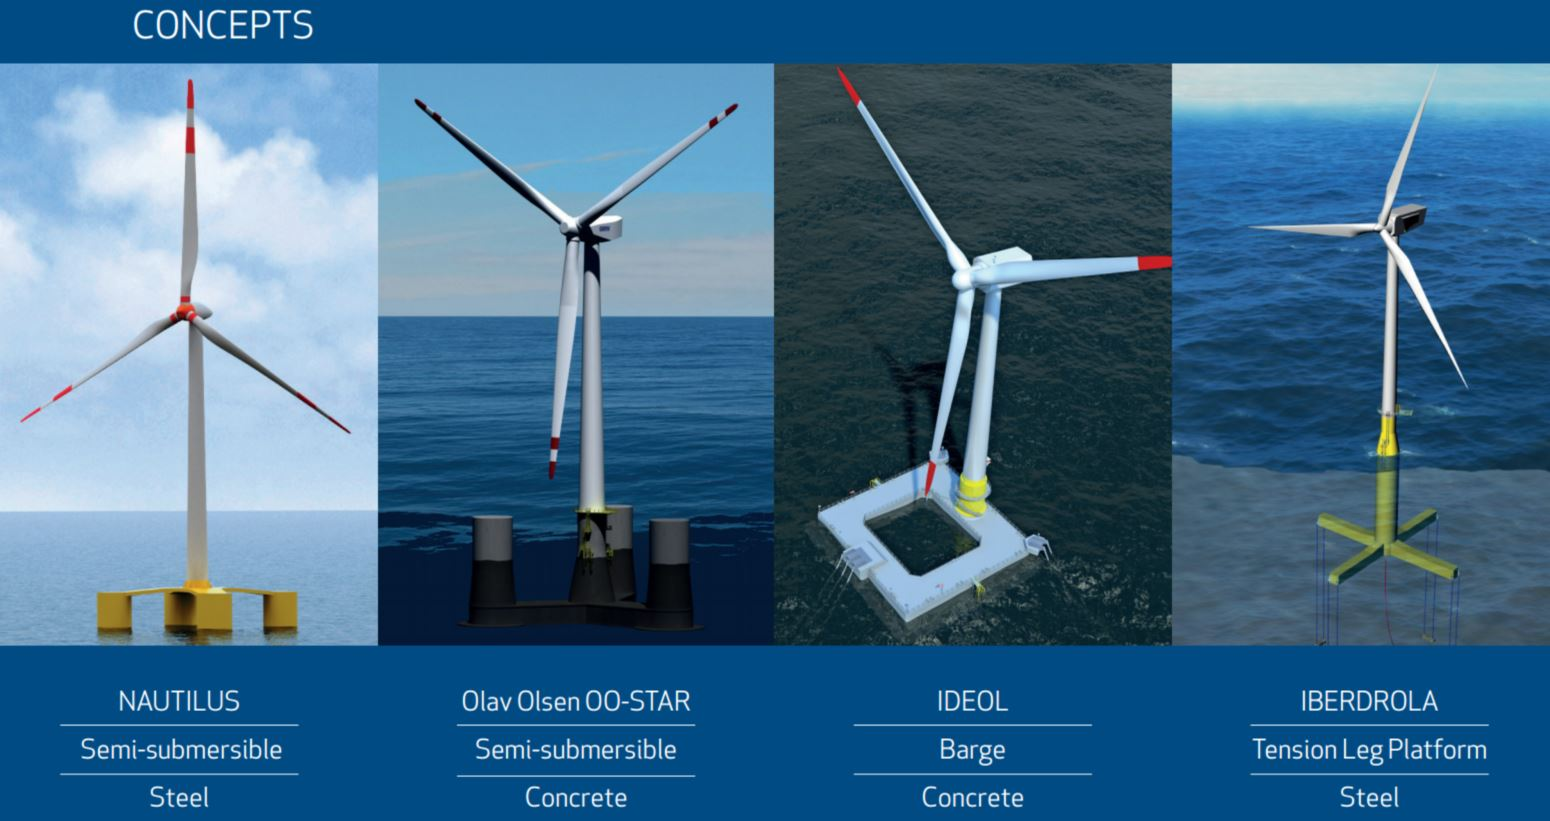
\includegraphics[scale=0.4]{figures/concepts}
\caption[$\; \:$Concepts of the Lifes50+ project]{The different concepts of the Lifes50+ project \cite{Lifes50+} }
 \label{fig:concept}
\end{figure}

\begin{figure}[H]
\centering
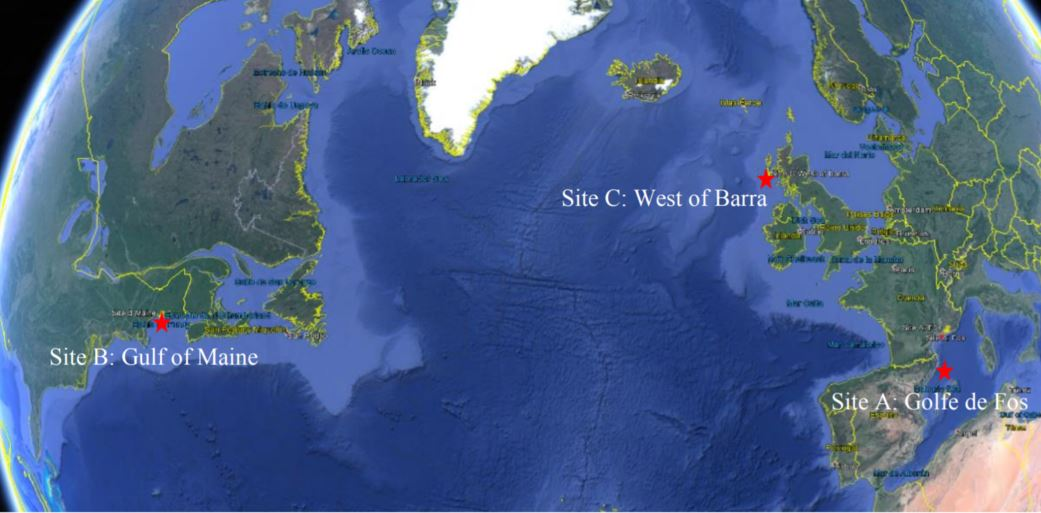
\includegraphics[scale=0.6]{figures/sites}
\caption[$\; \:$Sites for Lifes50+ project]{The different sites for Lifes50+ project, \cite{Lifes50+D1.6} }
 \label{fig:sites}
\end{figure}

\subsection{OO-Star}
OO-Star is one of the two designs to proceed to the second stage of the project. It is a design developed by the Norwegian company Dr. Techn. Olav Olsen.\newline
\newline
The support structure is a semi-submersible consisting of one column in the center supporting the tower and turbine, and three outer columns equally spaced, all mounted on a star-shaped pontoon, as can be seen in Figure \ref{fig:oostar}

\begin{figure}[H]
\centering
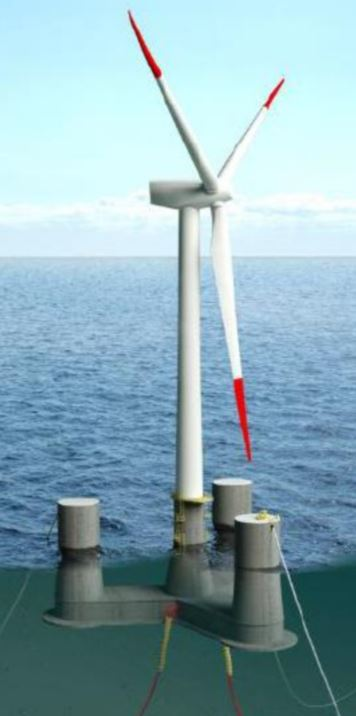
\includegraphics[scale=0.6]{figures/oostar}
\caption[$\; \:$Dr. Techn. Olav Olsen's OO-Star]{Dr. Techn. Olav Olsen's OO-Star \cite{Lifes50+D4.2} }
 \label{fig:oostar}
\end{figure}

\noindent The main material is post-tensioned concrete, and the main dimensions are displayed in Figure \ref{fig:designoostar}

\begin{figure}[H]
\centering
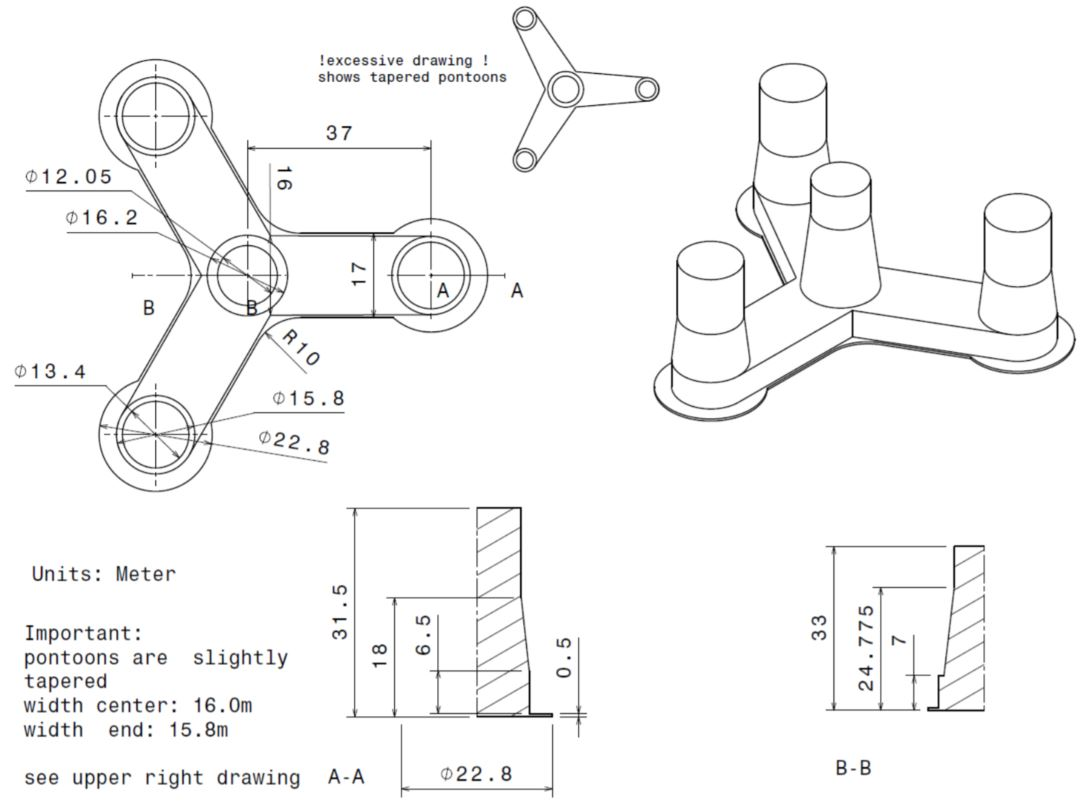
\includegraphics[scale=0.6]{figures/designoostar}
\caption[$\; \:$Main dimensions of OO-Star]{Main dimensions of OO-Star \cite{Lifes50+D4.2} }
 \label{fig:designoostar}
\end{figure}

\subsection{Wind Turbine Floater Motions}
To simulate the motion of OO-Star, Dr. Techn. Olav Olsen have provided the transfer functions for all 6 degrees of freedom of the vessel. The transfer functions are valid for the center of the model, however, the cable is attached some distance from the center of gravity as can be seen in Figure \ref{fig:cabhang}. This distance has been calculated to be 9.24m, and had to be taken into consideration in the modelling process. 

\begin{figure}[H]
\centering
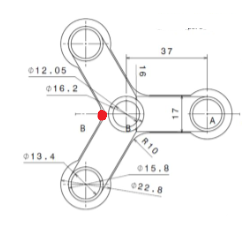
\includegraphics[scale=1.2]{figures/cabhang}
\caption[$\; \:$Cable hang off position]{Cable hang off position, modified from \cite{Lifes50+D4.2}}
 \label{fig:cabhang}
\end{figure}
 \noindent The transfer functions of OO-Star are confidential and can not be reproduced in this report. 
 
\section{Power Cable}
 The power cable used in this master thesis had three-phase AC circuits placed in one cable. The choice of power cable cross section was based on guidance from Professor Svein Sævik. 

\subsection{Cable Cross Section}
 An illustration of the model cross section used is shown in Figure \ref{fig:cross2}. 

\begin{figure}[H]
\centering
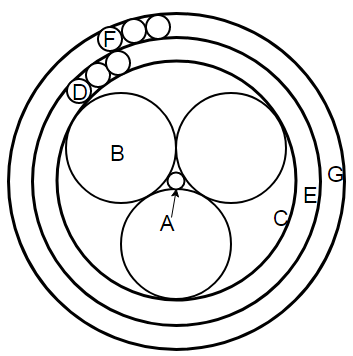
\includegraphics[scale=0.9]{figures/cross2}
\caption[$\; \:$Cable cross section in local model]{Illustration of cable cross section in local model  }
 \label{fig:cross2}
\end{figure}

\noindent The different components in the local model are:
\begin{enumerate}[label=\Alph*]
\item Center tube
\item Electrical conductor + insulation
\item Sheath around conductors
\item 1st layer of Armouring 
\item Tape between the two layers of armouring
\item 2nd layer of armouring
\item Protective sheath
\end{enumerate}

\noindent The dimensions of components of the cross-section are based on the conductor + insulation cross-section, and all other dimensions are calculated from this. The conductor itself has an area of 95$mm^2$, and in addition, there is a layer of insulation, making the radius of the of conductor + insulation 15mm.  The calculations of the radius of the center tube and the 1st sheath are based on trigonometry. By imagining a like-sided triangle with its corners in the center of each of the conductors, the following relations can be derived: 


  \begin{equation}
   r_{ct} = r_c (\tan(60)-\tan(30)-1)
\end{equation}

 \noindent Where $r_{ct}$ is the radius of the core and $r_c$ is the radius of the conductor.

 \begin{equation}
   r_{s} = r_c (1+\tan(60)-\tan(30))
\end{equation}
 
  \noindent Where $r_{s}$ is the radius of the sheath around the conductors and $r_c$ is the radius of the conductor. \newline
  \newline 
  \noindent The dimensions of the cable cross section are given in Table \ref{table:cabledim}, and were determined in agreement with Professor Svein Sævik.  


\begin{table} [H]
\centering
\begin{tabular}{ |c|c|c|}
\hline
Component & Radius [mm] & Thickness [mm] \\
 \hline
 \hline
 Conductor + Insulation & 15 &\\

 Center tube & 2.32& \\
 
 Sheath 1 & 33.07 & 1.5 \\
 
Armouring & 1.5 &  \\

Tape & 37.57 & 0.5 \\

Sheath 3 & 42.82& 3  \\

 \hline
\end{tabular}
\caption{Dimensions of local model}
\label{table:cabledim}
\end{table} 

\noindent There are 63 steel armouring fibers in the inner layer of the armouring, and 71 in the outer layer. This was calculated by the following expression:
\begin{equation}
    n_i=\frac{F_j\cos(\alpha)\pi D_c}{D_s}
\end{equation}
Where $F_j$ is the fill factor (0.9 was used), $\alpha$ is the lay angle (20 degrees was used), $D_c$ is the diameter of the cable and $D_s$ is the diameter of one steel fibre. 

\section{Environmental Conditions}
 This section contains information mainly from the report \cite{Lifes50+D1.1}.\\\\As mentioned earlier in this section, 3 possible locations were used for the Lifes50+ project with different degrees of challenging conditions. For this study, the chosen location was West of Barra, Scotland. The main basis for this choice was that this was the site with the deepest water, and this is also the site with the most challenging weather conditions. The exact proposed location was in the area with the coordinates 56.609$^\circ$N, 7.996$^\circ$W. 


\begin{figure}[H]
\centering
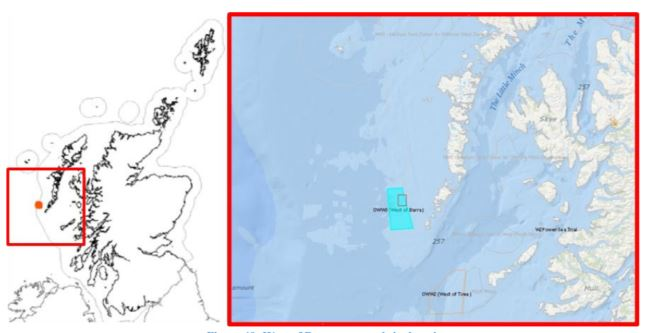
\includegraphics[scale=0.8]{figures/wob}
\caption[$\; \:$West of Barra, Scotland]{Possible location for floating wind turbine, West of Barra, Scotland \cite{Lifes50+D1.1} }
 \label{fig:wob}
\end{figure}

\noindent The water depth at the location West of Barra is between 56-118m, and 118m was used in this study.

\subsection{Wind Climate}
\label{sec:windcli}

The wind speeds at West of Barra are high and reliable throughout the year, with a mean annual power density of 1.3 $\frac{kW}{m^2}$. The following wind and wave data are based on \cite{geos2001}, and extrapolated and modified by \cite{Lifes50+D1.1}. 
\\\\
Table \ref{table:wind} shows the ten minute mean wind speed profile at different heights, and extreme value wind speed is shown in Table  \ref{table:windex}
\begin{table} [H]
\centering
\begin{tabular}{ |c|c|}
\hline
 Height [m]& Wind speed [m/s]\\
 \hline
 \hline
 10 & 9.50 \\

 20 & 10.16 \\
 
 50 & 10.97 \\
 
 120 & 11.58 \\

 119 & 11.74  \\
 \hline
\end{tabular}
\caption{Ten minute mean wind speed profile}
\label{table:wind}
\end{table}

\begin{table} [H]
\centering
\begin{tabular}{ |c|c|}
\hline
 Height [m]& Wind speed [m/s]\\
 \hline
 \hline
 10 & 26.47 \\

 20 & 35.63 \\
 
 50 & 44.13 \\
 
 120 & 48.97 \\

 119 & 50.00  \\
 \hline
\end{tabular}
\caption{Ten minute mean extreme value speed profile}
\label{table:windex}
\end{table}

\noindent Figure \ref{fig:scatterwind} shows the scatter diagram for wind conditions at west of Barra. With north being 0 degrees

\begin{figure}[H]
\centering
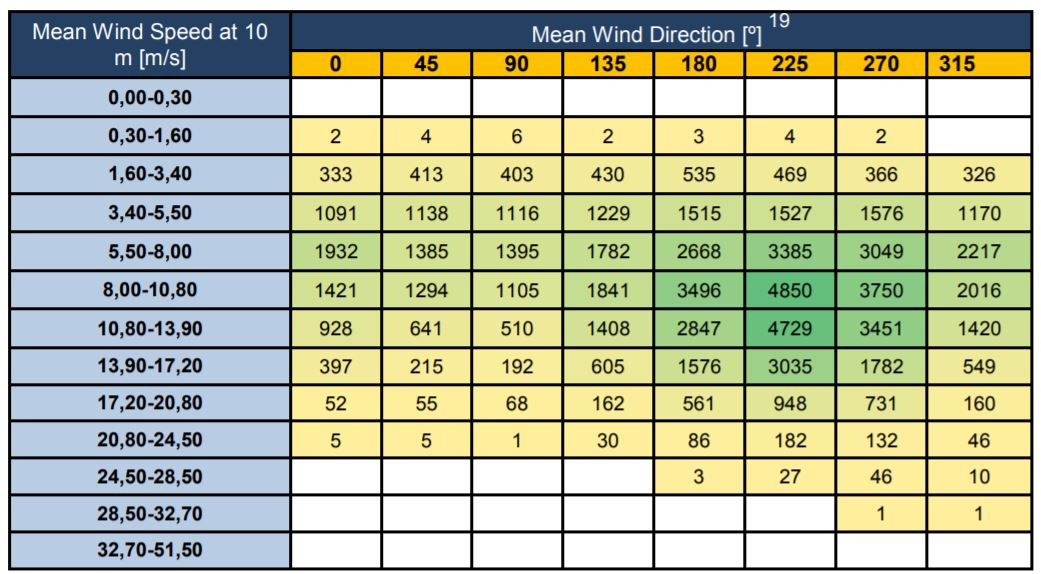
\includegraphics[scale=0.7]{figures/scatterwind}
\caption[$\; \:$Scatter diagram for wind conditions]{Scatter diagram for wind conditions at West of Barra \cite{Lifes50+D1.1} }
 \label{fig:scatterwind}
\end{figure}
 
 \noindent The max annual wind speed at 10 m above sea surface with 1-year return period is calculated by \cite{Lifes50+D1.1} to be  29.36 $\frac{m}{s}$



\subsection{Wave Climate}
The wave loads applied to the floating wind turbine were based on the scatter diagram for West of Barra. According to the transfer functions for heave, obtained from Dr.Techn. Olav Olsen, severe resonance in heave will occur at periods around 19s-24s in heave. As Tp is only the average of the 1/3 highest waves, resonance was observed for Tps lower than 19s in the global analyses. To avoid the area of severe resonance, an thus extreme response for the wind floater, the sea states for the periods 16 -17, 17-18 seconds and 18-19 seconds were moved to the 15-16 seconds column, and thus maintaining the total number of observations. The original and modified scatter diagrams can be seen in Figures \ref{fig:scato} and \ref{fig:scatn}.

\begin{figure}[H]
\centering
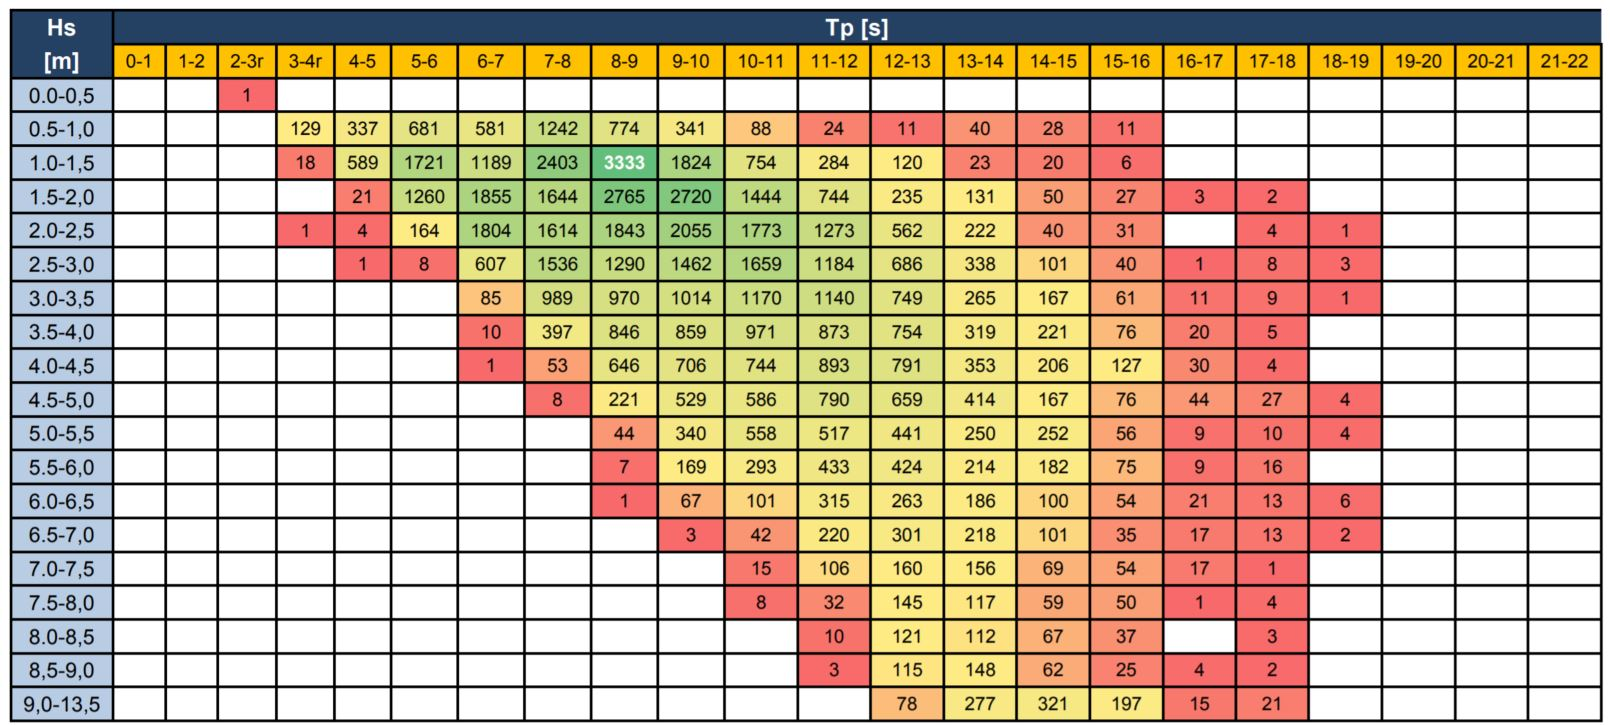
\includegraphics[scale=0.5]{figures/scatteroriginal}
\caption[$\; \:$Original scatter diagram]{Original scatter diagram \cite{Lifes50+D1.1} }
 \label{fig:scato}
\end{figure}

\begin{figure}[H]
\centering
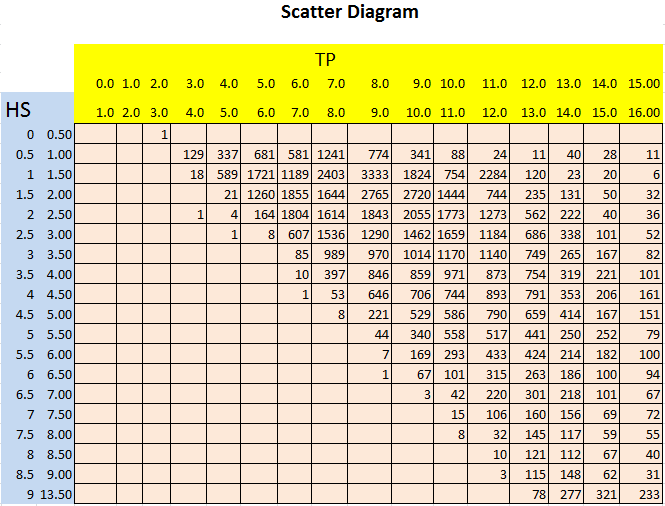
\includegraphics[scale=0.8]{figures/scatternew}
\caption[$\; \:$Modified scatter diagram ]{Modified scatter diagram  }
 \label{fig:scatn}
\end{figure}
 
 \noindent \cite{Lifes50+D1.1} states that there is no data on the correlation between the wind direction and the wave direction.
 \subsection{Current}
 \label{sec:current}
 According to \cite{Lifes50+D1.1}, the coast of Scotland is located on the UK Continental Shelf, so that it is directly affected by the oceanic circulations. However, the amount of water traveling from deep waters of the Atlantic sea to the shallower waters of the continental shelf is reduced due to the steepness of the slope of the shelf. Tidal currents are stronger and easier to predict than the non-tidal currents in the area. Winds, jets and density-driven currents affects the non-tidal currents strongly, and this may lead to large changes of the general current patterns for short periods. There are no specific data on the current conditions of West for Barra. However, according to \cite{dnvenviroment}, when detailed field measurements are missing, the current speed profile can be modelled with two components: wind generated current and tidal current. \newline
  \newline
  \subsubsection{Wind Generated Current}
  The wind induced current speed at still water level (z=0) can be calculated, if no statistical data is available, as:
  
  \begin{equation}
      V_{c,wind}(0)=k U_{1hour,10m}
  \end{equation}
  Where $k$ is a constant in range 0.015-0.03, and $U_{1hour,10m}$ is the 1 hour wind speed at height 10 m above sea level.\newline
  \newline
  By using $k=0.03$ and and 29.36$\frac{m}{s}$ as current speed at still water level (see section \ref{sec:windcli}, the current speed at still water level was calculated to:\newline
\newline
$$V_{c,wind}(0)=0.881$$   
  Then the current speed profile can be calculated as a linear profile from $d_0 < z < 0$:
  
  \begin{equation}
      V_{c,wind}(z)= V_{c,wind}(0) \left( \frac{d_0+z}{d_0}\right)
  \end{equation}
  
  \noindent Where $ V_{c,wind}(z)$ is the current speed at still water level, $d_0$ is the reference depth for wind generated current $d_0$=50m, and z is the distance from still water level, positive upwards. \newline
  \newline
  
\subsubsection{Deep Water Current } 
 The data in this section is taken from \cite{hseenironmental} and reproduced by \cite{Lifes50+D1.1}.\newline
   \newline
   The 50 year return period speed and directions for tidal current and storm surge current was found to be 0.44 m/s with North-East direction, and 0.6 m/s with North direction respectively. From this, the 1 year return period velocities could be calculated by a correction factor of 0.89. The combined velocity and direction was calculated as the vectorial sum.
   
   
\begin{table} [H]
\centering
\begin{tabular}{ |c|c|c|c|}
\hline
Return Period & Tidal Current & Storm Surge Current & Combined Current \\
 \hline
 \hline
 & Vc[m/s] \hspace{0.3cm} Dir[$^{\circ}$] &  Vc[m/s] \hspace{0.3cm} Dir[$^{\circ}$] & Vc[m/s] \hspace{0.3cm} Dir[$^{\circ}$] \\
 \hline
 1 & 0.39 \hspace{0.7cm} 50 & 0.53 \hspace{0.7cm} 0  & 0.84 \hspace{0.7cm} 21 \\
 50 & 0.44 \hspace{0.7cm} 50 & 0.60 \hspace{0.7cm} 0  & 0.94 \hspace{0.7cm} 21 \\
 \hline
\end{tabular}
\caption{Deep Water Current at Sea Surface, reproduced from \cite{Lifes50+D1.1}}
\label{table:tidcur}
\end{table} 

\noindent According to \cite{dnvenviroment}, the 1 year return period data from Table \ref{table:tidcur} can be used to calculate the tidal and storm surge current profile for $z \leq 0$:

 \begin{equation}
      V_{c,tide}(z)= V_{c,tide}(0) \left( \frac{d+z}{d_0}\right)^{\alpha}
  \end{equation}
  
  \noindent Where $ V_{c,tide}(z)$ is the current speed at still water level, $d$ is the water depth to still water level (taken positive), and z is the distance from still water level, positive upwards, $\alpha$ is the exponent, typically $\alpha = \frac{1}{7}$

   \subsubsection{Current Speed Profile}
  As a simplification, only three different weather conditions are considered: 
  \begin{itemize}
      \item Far: Wind direction and wind induced current direction is the same as wave direction
     \item Neutral: No wind, only tide and storm surge current
     \item Near:  Wind direction and wind induced current direction is the opposite to wave direction
  \end{itemize}
 The current profiles for the three weather conditions were calculated as the vectorial sum of the wind induced current and the tidal- and storm surge current. The profiles are displayed in Tables \ref{table:tidcurnear} to \ref{table:tidcurfar}, where north is defined as 0$^{\circ}$:  
\begin{table} [H]
\centering
\begin{tabular}{ |c|c|c|c|}
\hline
Depth [m] & Wind & Tidal and Surge & Total Current Profile \\
 \hline
 \hline
 & Vc[m/s] \hspace{0.3cm} Dir[$^{\circ}$] &  Vc[m/s] \hspace{0.3cm} Dir[$^{\circ}$] & Vc[m/s] \hspace{0.3cm} Dir[$^{\circ}$] \\
 \hline
 0 & 0.881 \hspace{0.7cm} 270 & 1.023 \hspace{0.7cm} 21  & 1.085 \hspace{0.7cm} 331.70 \\
 -10 & 0.705 \hspace{0.7cm} 270 & 1.008 \hspace{0.7cm} 21  & 1.010 \hspace{0.7cm} 340.49 \\
 -20 & 0.528 \hspace{0.7cm} 270 & 0.992 \hspace{0.7cm} 21  & 0.942
 \hspace{0.7cm} 349.47 \\
 -30 & 0.352 \hspace{0.7cm} 270 & 0.973 \hspace{0.7cm} 21  & 0.908 \hspace{0.7cm} 364.79 \\
 -40 & 0.176 \hspace{0.7cm} 270 & 0.952 \hspace{0.7cm} 21  & 0.904 \hspace{0.7cm} 10.48 \\
 -50 & 0.0 \hspace{0.7cm} - & 0.928 \hspace{0.7cm} 21  & 0.928 \hspace{1.15cm} 21 \\
  -60 & 0.0 \hspace{0.7cm} - & 0.900 \hspace{0.7cm} 21  & 0.900 \hspace{1.15cm} 21 \\
 -70 & 0.0 \hspace{0.7cm} - & 0.864 \hspace{0.7cm} 21  & 0.864 \hspace{1.15cm} 21 \\
  -80 & 0.0 \hspace{0.7cm} - & 0.817 \hspace{0.7cm} 21  & 0.817 \hspace{1.15cm} 21 \\
 -90 & 0.0 \hspace{0.7cm} - & 0.741 \hspace{0.7cm} 21  & 0.741 \hspace{1.15cm} 21 \\ 
 -100 & 0.0 \hspace{0.7cm} - & 0.0 \hspace{0.7cm} -  & 0.0 \hspace{1.15cm} - \\ 
 \hline
\end{tabular}
\caption{Current Speed and Direction Profile for Near wind condition, partly from \cite{Lifes50+D1.1}}
\label{table:tidcurnear}
\end{table}   

\begin{table} [H]
\centering
\begin{tabular}{ |c|c|c|c|}
\hline
Depth [m] & Wind & Tidal and Surge & Total Current Profile \\
 \hline
 \hline
 & Vc[m/s] \hspace{0.3cm} Dir[$^{\circ}$] &  Vc[m/s] \hspace{0.3cm} Dir[$^{\circ}$] & Vc[m/s] \hspace{0.3cm} Dir[$^{\circ}$] \\
 \hline
 0 & 0.0 \hspace{0.7cm} - & 1.023 \hspace{0.7cm} 21  & 1.023 \hspace{0.7cm} 21 \\
 -10 & 0.0 \hspace{0.7cm} - & 1.008 \hspace{0.7cm} 21  & 1.008 \hspace{0.7cm} 21 \\
 -20 & 0.0 \hspace{0.7cm} - & 0.992 \hspace{0.7cm} 21  & 0.992
 \hspace{0.7cm} 21 \\
 -30 & 0.0 \hspace{0.7cm} - & 0.973 \hspace{0.7cm} 21  & 0.973 \hspace{0.7cm} 21 \\
 -40 & 0.0 \hspace{0.7cm} - & 0.952 \hspace{0.7cm} 21  & 0.952 \hspace{0.7cm} 21 \\
 -50 & 0.0 \hspace{0.7cm} - & 0.928 \hspace{0.7cm} 21  & 0.928 \hspace{0.7cm} 21 \\
  -60 & 0.0 \hspace{0.7cm} - & 0.900 \hspace{0.7cm} 21  & 0.900 \hspace{0.7cm} 21 \\
 -70 & 0.0 \hspace{0.7cm} - & 0.864 \hspace{0.7cm} 21  & 0.864 \hspace{0.7cm} 21 \\
  -80 & 0.0 \hspace{0.7cm} - & 0.817 \hspace{0.7cm} 21  & 0.817 \hspace{0.7cm} 21 \\
 -90 & 0.0 \hspace{0.7cm} - & 0.741 \hspace{0.7cm} 21  & 0.741 \hspace{0.7cm} 21 \\ 
 -100 & 0.0 \hspace{0.7cm} - & 0.0 \hspace{0.7cm} -  & 0.0 \hspace{0.7cm} - \\ 
 \hline
\end{tabular}
\caption{Current Speed and Direction Profile for Neutral wind condition, partly from \cite{Lifes50+D1.1}}
\label{table:tidcurneu}
\end{table}   

\begin{table} [H]
\centering
\begin{tabular}{ |c|c|c|c|}
\hline
Depth [m] & Wind & Tidal and Surge & Total Current Profile \\
 \hline
 \hline
 & Vc[m/s] \hspace{0.3cm} Dir[$^{\circ}$] &  Vc[m/s] \hspace{0.3cm} Dir[$^{\circ}$] & Vc[m/s] \hspace{0.3cm} Dir[$^{\circ}$] \\
 \hline
 0 & 0.881 \hspace{0.7cm} 90 & 1.023 \hspace{0.7cm} 21  & 1.571 \hspace{0.7cm} 52.56 \\
 -10 & 0.705 \hspace{0.7cm} 90 & 1.008 \hspace{0.7cm} 21  & 1.421 \hspace{0.7cm} 48.57 \\
 -20 & 0.528 \hspace{0.7cm} 90 & 0.992 \hspace{0.7cm} 21  & 1.279
 \hspace{0.7cm} 43.65 \\
 -30 & 0.352 \hspace{0.7cm} 90 & 0.973 \hspace{0.7cm} 21  & 1.147 \hspace{0.7cm} 37.64 \\
 -40 & 0.176 \hspace{0.7cm} 90 & 0.952 \hspace{0.7cm} 21  & 1.029 \hspace{0.7cm} 30.19 \\
 -50 & 0.0 \hspace{0.7cm} - & 0.928 \hspace{0.7cm} 21  & 0.928 \hspace{1.15cm} 21 \\
  -60 & 0.0 \hspace{0.7cm} - & 0.900 \hspace{0.7cm} 21  & 0.900 \hspace{1.15cm} 21 \\
 -70 & 0.0 \hspace{0.7cm} - & 0.864 \hspace{0.7cm} 21  & 0.864 \hspace{1.15cm} 21 \\
  -80 & 0.0 \hspace{0.7cm} - & 0.817 \hspace{0.7cm} 21  & 0.817 \hspace{1.15cm} 21 \\
 -90 & 0.0 \hspace{0.7cm} - & 0.741 \hspace{0.7cm} 21  & 0.741 \hspace{1.15cm} 21 \\ 
 -100 & 0.0 \hspace{0.7cm} - & 0.0 \hspace{0.7cm} -  & 0.0 \hspace{1.15cm} - \\ 
 \hline
\end{tabular}
\caption{Current Speed and Direction Profile for Far wind condition, partly from \cite{Lifes50+D1.1}}
\label{table:tidcurfar}
\end{table} 

\section{SN Fatigue Data}
To estimate the life time of the power cable, the S-N curve in Figure \ref{fig:snplot} was used. 

\begin{figure}[H]
\centering
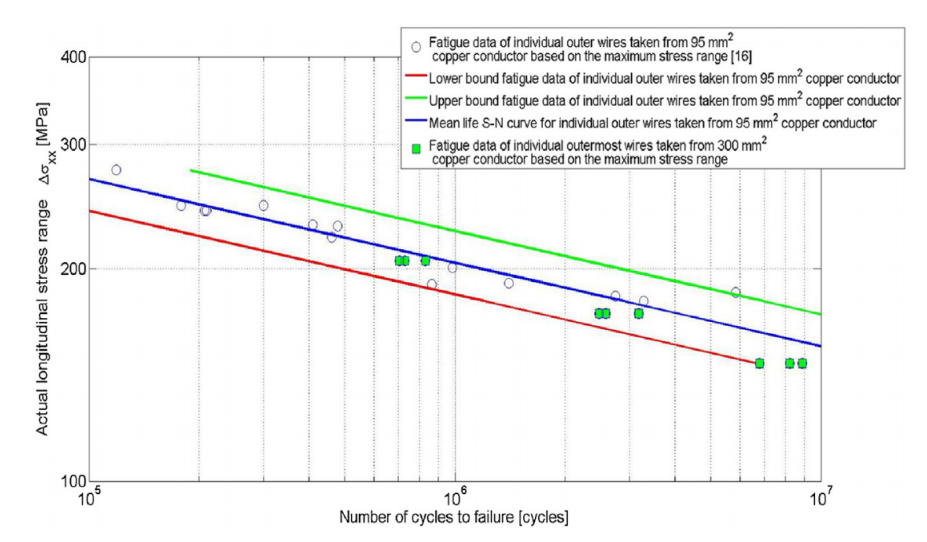
\includegraphics[scale=0.6]{figures/SNplot}
\caption[$\; \:$S-N data]{S-N data for case scenario,\cite{s300} }
 \label{fig:snplot}
\end{figure}
\noindent The blue S-N curve follows the log-linear relationship of Equation \ref{eq:sn}, with m=8.424 and c=2.88e25  according to \cite{Nasution2013}. The red plot is the S-N curve with two standard deviations subtracted, and was used in this study. The constants of the red plot are m=8.424 and c=1.57e25. 